% !TEX root = ../thesis.tex

Although hypothetically CORE offers a base that supports multiple modeling languages, only one notation has been integrated with CORE thus far---the RAM modeling notation that is used for design modeling with class, sequence, and state diagrams~\cite{kienzle2010aspect, klein2007reusable}. The goal of the thesis is to investigate whether CORE can also support an additional modeling language---the requirements specification language, specifically UCM for functional requirements modeling.

This chapter presents the corification of UCM using the CORE metamodel. We describe the steps taken to corify UCM in Section~\ref{sec:3.1}, in addition to tailor the customization and usage interfaces for UCMs. We also define the weaving algorithm specific for UCM in the context of CORE, fulfilling the needs of a requirements engineer to build modular UCMs using CORE model extensions and reuses, in Section~\ref{sec:3.2}.

\section{Corification of UCM} \label{sec:3.1}

The idea behind integrating a modeling language with CORE is to allow CORE concerns the ability to contain models of that language. This motivates us to investigate the possibility for UCMs to be part of the concerns, such that scenario models built with UCMs can serve as realization models for features of the concerns. To add support for CORE for a particular modeling language, the initial step is to first define the base metamodel for the language, and then derive the appropriate metaclasses from the CORE metamodel for CORE to recognize the language.

Abstract and concrete classes of the CORE metamodel are utilized differently when corifying a modeling language. The abstract classes \textit{\cls COREModel}, \textit{\cls COREModelElement}, and \textit{\cls COREPattern} serve as extension points and are intended to be subclassed by a modeling language. This enables the addition of arbitrary modeling languages to CORE and also uniform treatment of pattern-based composition. The remaining abstract classes \textit{\cls COREModelComposition}, \textit{\cls COREModelElementComposition}, and \textit{\cls CORELink} are used within the CORE metamodel and seldom subclassed by a modeling language. On the contrary, concrete classes are designed to be used exactly as it is in the corified modeling languages. They provide the necessary mechanisms for model extensions and reuses, feature and impact modeling, as well as a way to implements and visualizes these concepts in its modeling tool.

\begin{figure}
	\centering
	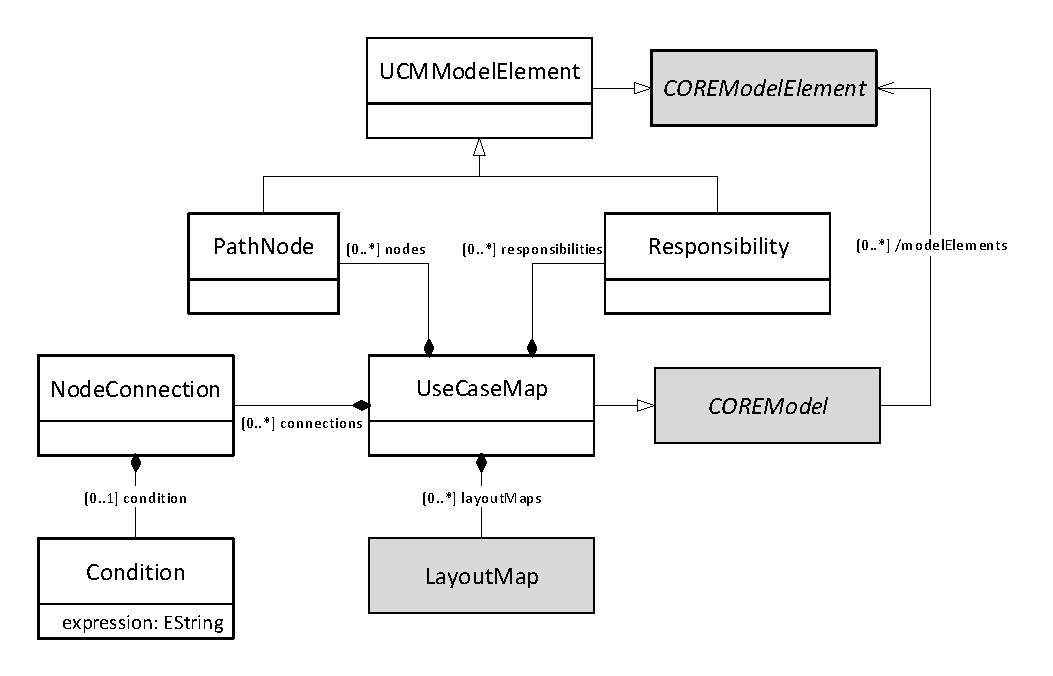
\includegraphics[scale=0.5]{fig_3_1.pdf}
	\caption{Extended UCM metamodel with CORE}
	\label{fig:3.1}
\end{figure}

We follow the URN specification~\cite{itu2012151} closely in corifying the UCM metamodel. Figure~\ref{fig:3.1} shows a partial view of the corified UCM metamodel, focusing on the elements that extend the CORE metamodel through subclassing (from an existing metaclass in the modeling language to an abstract CORE metaclass \footnote{The gray elements in the figures are the classes that derived from the CORE metamodel.}). By subclassing the necessary abstract classes of the CORE metamodel, UCM is able to provide all the properties of CORE:

\begin{enumerate}
	\setlength{\parskip}{0pt} \setlength{\itemsep}{0pt}
	\item A UCM model may now belong to a concern by realizing at least one of its features.
	\item A UCM realization model may now have impacts on high-level goals.
	\item A UCM model may extend another UCM model that belongs to a different feature.
	\item A UCM model may reuse another UCM model that belongs to a different concern.
\end{enumerate}

The first and second properties are achieved once the UCM metamodel is properly extended, since CORE provides feature and goal modeling by default to all supported realization models. The third and forth properties, however, requires some thought on determining the customization interface that best suites UCMs, as customization interface is unique to all corified modeling languages and mappings should be tailored to each of the languages. After much deliberation, we arrived at a decision to provide mappings of different UCM model elements based on CORE model extensions and CORE model reuses.

Since the most common unit of occurrence for UCMs is responsibility that represents much of the actions in use cases, one of the most likely candidates for mapping is the responsibility element and is especially useful for model extensions. Aspect-oriented modeling can be carried out by combining separate UCM paths together, with mapped responsibilities act as join points. To illustrate the concept, we take home security concern as an example, with the base scenario having at least a "lock" responsibility that represents an action to lock the door of the home before leaving. Consider an optional feature "alarm system" that might be added to the home security. A typical UCM would use a stub, along with OR-forks and OR-joins, to model the optional feature in the root UCM. This, however, results in "alarm system" tangled up with the root UCM. Our approach resolves this issue by shifting the need to specify join points to the optional feature itself, by mapping responsibilities between the parent and child UCMs. In this case, we would also have a "lock" responsibility in the UCM that models the "alarm system" feature, and model the alarm system scenario (e.g., "enter code" and "validate code") prior to "lock", then map the "lock" responsibilities between the root UCM and feature UCM. We simply augment the base scenario through model extension, so whenever the feature "alarm system" is selected as part of the home security, the model would include the scenario for setting up the alarm system as modeled in the "alarm system" feature after composing all the necessary models together. Otherwise if "alarm system" is not selected, the composed model would only have the locking mechanism without any model elements that represent the alarm system tangled up with the root UCM.

The idea of having a stub to represent a container for reusing UCM models is straightforward. Because the purpose of a stub is to bind plug-ins that consists of separate UCMs, a UCM model that is being reused can appear as a plug-in for the stub. Whereas the start and end points of the plug-ins connect the path segments coming in and going out of a stub to form the continuation of paths between the stub and plug-ins, similarly the start and end points of the reused UCM model connect the path segments coming in and going out of a stub. Reusing a UCM model is essentially reusing a concern---the selection of features when reusing a concern determines the final UCM model to be reused.

Reusing a concern from a UCM model prompts the feature selection process. This signals the feature that the UCM model realizes to reuse the other concern with the desired feature(s). The reusing UCM model then establishes the mappings to the reused UCM model that realizes the reused features. This is achieved as follows. The root element {\cls UseCaseMap} subclasses \textit{\cls COREModel}, which makes it part of a {\cls COREConcern} (see Figure~\ref{fig:2.1}, association between {\cls COREConcern} and {\cls COREModel}). This allows a UCM to realize a feature (see Figure~\ref{fig:2.2}, {\cls COREModel} realizes {\cls COREFeature}) within a concern. Therefore, the concern can create a {\cls COREReuse} to reuse another concern. The reusing UCM then creates a {\cls COREModelReuse} that has a direct association to the created {\cls COREReuse} and a \textit{\cls COREConfiguration} that selects the desired features from the reused concern. The CORE modeling tool then composes the UCM models of the reused concern that realize the selected features to generate a single woven user-tailored UCM model of the reused concern. Mappings to the model elements of this generated model are established using the class {\cls COREMapping}, consequently allowing the reusing UCM to customize the generated UCM model of the reused concern.

\begin{figure}
	\centering
	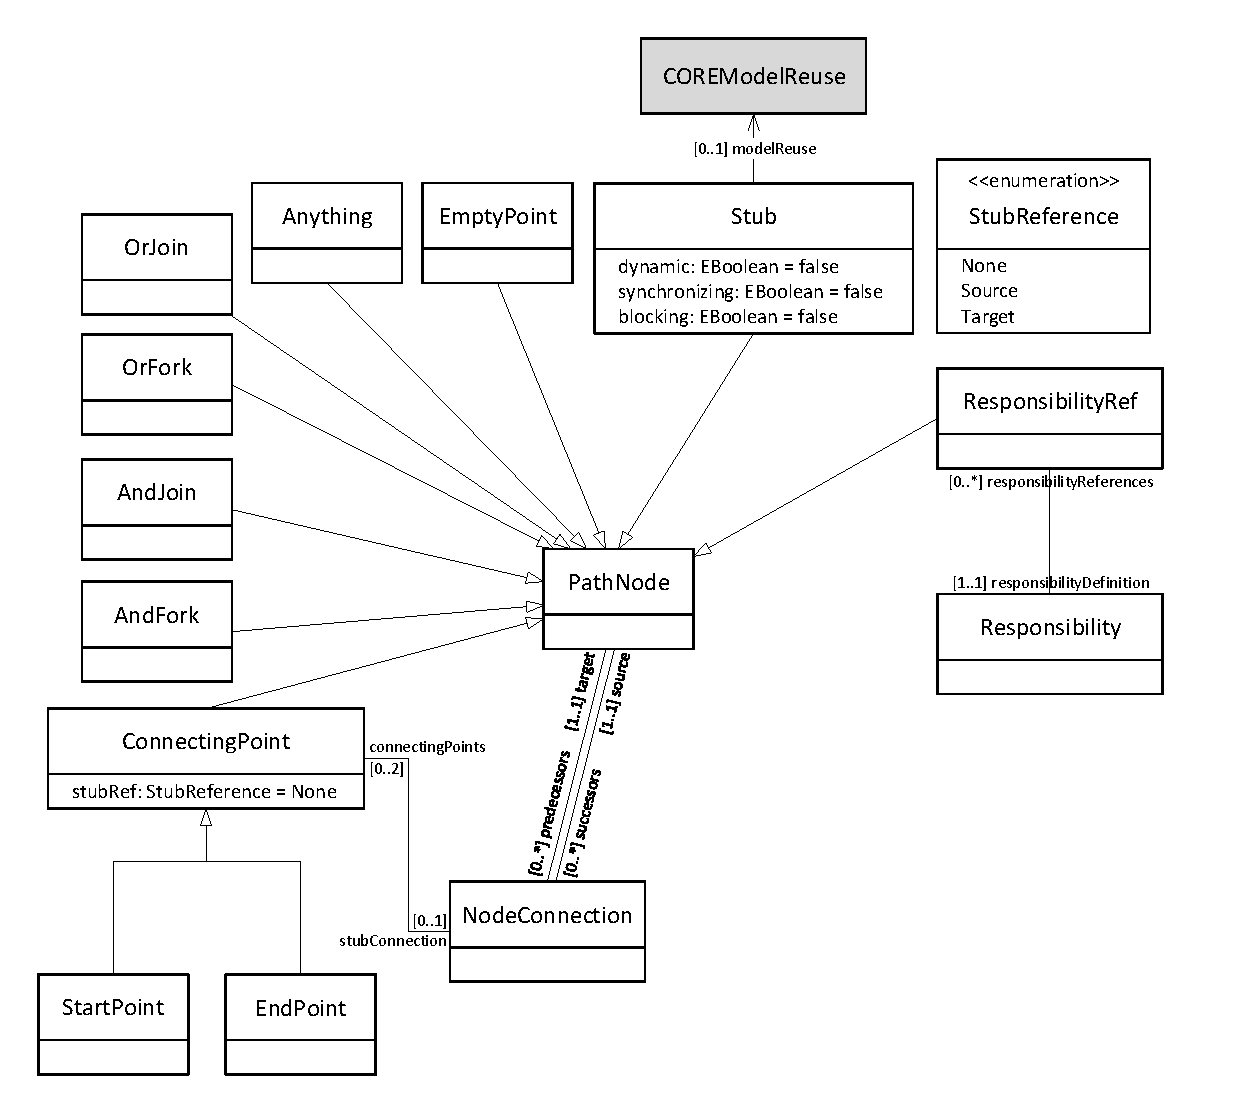
\includegraphics[scale=0.5]{fig_3_2.pdf}
	\caption{Path nodes for corified UCM}
	\label{fig:3.2}
\end{figure}

A standard UCM consists of {\cls PathNode}, {\cls Responsibility}, and {\cls NodeConnection}. {\cls LayoutMap} is added as part of the composition to allow positioning of the elements for viewing. We omit the inclusion of certain elements such as {\cls Component}, {\cls Timer}, and {\cls FailurePoint} to limit the scope of this thesis. On the contrary, {\cls PluginBinding} is excluded on purpose since we utilize {\cls COREMapping} as our approach to bind separate UCMs to {\cls Stub}. We incorporate several changes to the path nodes to support aspect-oriented modeling and reuse. Figure~\ref{fig:3.2} illustrates the addition of {\cls Anything} and {\cls ConnectingPoint}, as well as a directed association from {\cls Stub} to {\cls COREModelReuse}, to the UCM metamodel.

\textbf{\cls Anything:} We included the {\cls Anything} pointcut element from the extended AoUCM metamodel~\cite{mussbacher2011aspect}. {\cls Anything} (denoted by \textbf{\ldots}) acts as a wild card and can represent a subset of nodes in a path to allow variations in pattern matching. This is useful for facilitating complex model weaving, as it allows any sequence of UCM model elements, including an empty sequence, to be matched. Similar to the pointcut elements of sequence diagram in RAM~\cite{kienzle2009aspect}, the pointcut of an object lifeline represented with a *-box refers to the matched behavior of an advised sequence diagram, whereas the pointcut of a message labeled with a * means that any message between two objects is of interest.

\textbf{\cls ConnectingPoint:} We established a new path element to the metamodel. {\cls ConnectingPoint} is used to replace {\cls PluginBinding} and serves as an intermediate node that represents either a {\cls StartPoint} or an {\cls EndPoint}. By default, an actual start or end point within a UCM does not have a reference to a stub, hence the default value for {\cls StubReference} is {\cls None}. Instead, when we have a {\cls NodeConnection} that connects an element with a stub, then a hidden connecting point is automatically attached to the node connection (and deleted upon removal of the connection). Each node connection can have at most two connecting points if both the predecessor and successor nodes of the connection are stubs. Incoming connection to a stub generates a hidden end point with the value of {\cls stubRef} set to {\cls Target}, whereas outgoing connection from a stub generates a hidden start point with the value of {\cls stubRef} set to {\cls Source}. These hidden points allow us to define composition specifications through customization mappings.

\begin{figure}
	\centering
	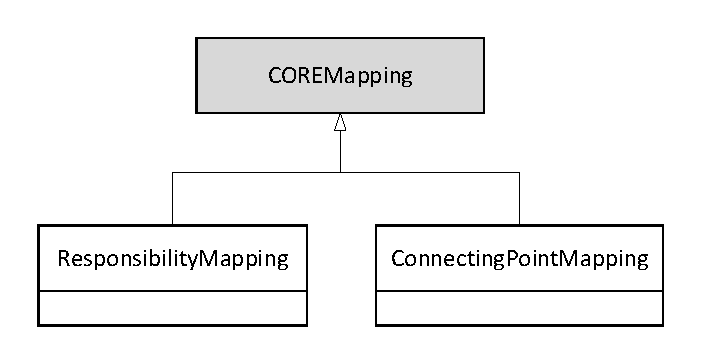
\includegraphics[scale=0.5]{fig_3_3.pdf}
	\caption{Customization mappings for corified UCM}
	\label{fig:3.3}
\end{figure}

Since we are using {\cls COREMapping} to specify customizations, it is necessary for {\cls UCMModelElement} to subclass \emph{\cls COREModelElement}. That way, all subclasses of {\cls UCMModelElement} (i.e., {\cls PathNode} and {\cls Responsibility}) can be used as source and destination classes for {\cls COREMapping}. As shown in Figure~\ref{fig:3.3}, we defined the composition specifications for specific UCM model elements: {\cls Responsibility} and {\cls ConnectingPoint}. They were selected so that we can compose UCM models based on the mappings of these elements. This leads us to the next section where we describe in detail how model composition is achieved through weaving.

\section{UCM Weaving} \label{sec:3.2}

The role of the weaver is to facilitate model extensions and reuses. We offer two options when mapping elements between UCMs: (i) direct mapping of responsibilities; and (ii) cross mapping of connecting points. Cross mapping is necessary because of the nature of start and end points, where a start point of a UCM maps to an end point of a stub, and vice versa. A stub can be perceived as being superimposed with an end point followed by a start point, and those points collapsed into a point that is the stub \cite{buhr1995use}. Here, the hidden end point of a stub represents the incoming connection and it signifies the end of the sequence before the stub, and the hidden start point of a stub represents the outgoing connection and it signifies the start of the sequence after the stub. Both options have different procedures when weaving.

\subsection{Weaving Algorithm}

As explained in Section~\ref{sec:2.1.2}, CORE models are always composed in pairs with \emph{single weave}, and complex extension and reuse hierarchies are usually composed with multiple levels of single weaves. The algorithms presented here are specific for single weaving, meaning that a composition is performed from one model (\emph{UCM}\textsubscript{source}) to another model (\emph{UCM}\textsubscript{target}). This action can be chained together with other compositions, even with the hierarchical structure of the concern features. Here, we specify the subscript \textsubscript{source} for the model elements of a UCM the weaver composes from, and the subscript \textsubscript{target} for the model elements of a UCM the weaver composes to. \emph{UCM}\textsubscript{source} and \emph{UCM}\textsubscript{target} are merged prior to weaving, retaining all the path nodes and node connections from both models. Then the weaver iterates through the available composition specifications and executes the algorithms based on the specific type of mapping. The output of the woven model results in the amalgamation of UCMs based on the composition specification defined by the designer of the models, as well as the selected features of the concern by the user.

\subsubsection{Responsibility Mapping} \label{sec:3.2.1.1}

\begin{algorithm}
    \caption{Weaving Algorithm: Responsibility Mapping}
    \label{alg:1}
	\begin{algorithmic}[1]
	    \Function{WeaveResponsibilityMapping}{\emph{ucm}, \emph{composition}}
			\State \emph{node}\textsubscript{source} $\gets$ get first node of \emph{composition} mapping (\emph{from})
			\State \emph{node}\textsubscript{target} $\gets$ get second node of \emph{composition} mapping (\emph{to})
			\State mark \emph{node}\textsubscript{target} as visited
			\State indicate start point has not been encountered
			\State indicate end point has not been encountered
			\State call \Call{TraverseToPredecessor}{\emph{ucm}, \emph{node}\textsubscript{target}, \emph{node}\textsubscript{source}}
			\State call \Call{TraverseToSuccessor}{\emph{ucm}, \emph{node}\textsubscript{target}, \emph{node}\textsubscript{source}}
			\State remove \emph{node}\textsubscript{source} from \emph{ucm}
		\EndFunction
		
		\Function{TraverseToPredecessor}{\emph{ucm}, \emph{node}\textsubscript{target}, \emph{node}\textsubscript{source}}
			\For{each predecessor of \emph{node}\textsubscript{target}}
				\State \emph{node}\textsubscript{target\textsubscript{pred}} $\gets$ get predecessor of \emph{node}\textsubscript{target}
				\If{linkage exists from previous mapping} \label{alg:1.1}
					\State set the predecessor of \emph{node}\textsubscript{target}'s connection to \emph{node}\textsubscript{source}'s predecessor
					\State disable linkage
					\State skip this loop
				\EndIf \label{alg:1.2}
				\If{\emph{node}\textsubscript{target\textsubscript{pred}} is visited} \label{alg:1.3}
					\State skip this loop
				\ElsIf{\emph{node}\textsubscript{target\textsubscript{pred}} is not {\cls Anything}}
					\State mark \emph{node}\textsubscript{target\textsubscript{pred}} as visited
				\EndIf \label{alg:1.4}
				\If{\emph{node}\textsubscript{target\textsubscript{pred}} is {\cls StartPoint} and start point is not encountered} \label{alg:1.5}
					\If{visibility of \emph{node}\textsubscript{target\textsubscript{pred}} is {\cls Concern}}
						\State set the predecessor of \emph{node}\textsubscript{target}'s connection to \emph{node}\textsubscript{source}'s predecessor
						\State remove \emph{node}\textsubscript{target\textsubscript{pred}} from \emph{ucm}
						\State indicate start point has been encountered
					\EndIf \label{alg:1.6}
				\ElsIf{\emph{node}\textsubscript{target\textsubscript{pred}} is {\cls Anything}} \label{alg:1.7}
					\State set the predecessor of \emph{node}\textsubscript{target}'s connection to \emph{node}\textsubscript{source}'s predecessor
					\If{\emph{node}\textsubscript{target\textsubscript{pred}} does not have any predecessor}
						\State remove \emph{node}\textsubscript{target\textsubscript{pred}} from \emph{ucm}
					\EndIf \label{alg:1.8}
				\Else
					\State recursively call \Call{TraverseToPredecessor}{\emph{ucm}, \emph{node}\textsubscript{target\textsubscript{pred}}, \emph{node}\textsubscript{source}} \label{alg:1.9}
				\EndIf
			\EndFor
		\EndFunction
		
		\algstore{alg1}
	\end{algorithmic}
\end{algorithm}

\begin{algorithm}                     
	\begin{algorithmic}[1]
		\algrestore{alg1}
		
		\Function{TraverseToSuccessor}{\emph{ucm}, \emph{node}\textsubscript{target}, \emph{node}\textsubscript{source}}
			\For{each successor of \emph{node}\textsubscript{target}}
				\State \emph{node}\textsubscript{target\textsubscript{succ}} $\gets$ get successor of \emph{node}\textsubscript{target}
				\If{\emph{node}\textsubscript{target\textsubscript{succ}} is visited} \label{alg:1.10}
					\State skip this loop
				\ElsIf{\emph{node}\textsubscript{target\textsubscript{succ}} is not {\cls Anything}}
					\State mark \emph{node}\textsubscript{target\textsubscript{succ}} as visited
				\EndIf \label{alg:1.11}
				\If{\emph{node}\textsubscript{target\textsubscript{succ}} is {\cls Endpoint} and end point is not encountered} \label{alg:1.12}
					\If{visibility of \emph{node}\textsubscript{target\textsubscript{succ}} is {\cls Concern}}
						\State set the successor of \emph{node}\textsubscript{target}'s connection to \emph{node}\textsubscript{source}'s successor
						\State remove \emph{node}\textsubscript{target\textsubscript{succ}} from \emph{ucm}
						\State indicate end point has been encountered
					\EndIf \label{alg:1.13}
				\ElsIf{\emph{node}\textsubscript{target\textsubscript{succ}} is {\cls Anything}} \label{alg:1.14}
					\State set the successor of \emph{node}\textsubscript{target}'s connection to \emph{node}\textsubscript{source}'s successor
					\If{\emph{node}\textsubscript{target\textsubscript{succ}} does not have any successor}
						\State remove \emph{node}\textsubscript{target\textsubscript{succ}} from \emph{ucm}
					\EndIf \label{alg:1.15}
				\ElsIf{\emph{node}\textsubscript{target\textsubscript{succ}} exists in \emph{composition} mapping (\emph{to})} \label{alg:1.16}
					\State copy node connection of successor
					\State set the successor of copied connection to \emph{node}\textsubscript{source}'s successor
					\State add the copied connection to \emph{ucm}
					\State enable linkage to next mapping \label{alg:1.17}
				\Else
					\State recursively call \Call{TraverseToSuccessor}{\emph{ucm}, \emph{node}\textsubscript{target\textsubscript{succ}}, \emph{node}\textsubscript{source}} \label{alg:1.18}
				\EndIf
			\EndFor
		\EndFunction
	\end{algorithmic}
\end{algorithm}

Mapping with responsibilities allows for model extensions between parent and child UCMs. Composition specification can be defined by mapping from a parent UCM's responsibility to a child UCM's responsibility. The idea is to insert the paths defined in the child UCM to the appropriate position in the parent UCM based on the mappings. We take a simple UCM in Figure~\ref{fig:3.4} as a base scenario for extension examples. Algorithm~\ref{alg:1} illustrates the procedure of weaving for responsibility mappings. The function \emph{WeaveResponsibilityMapping} initiates the process by identifying the mapped responsibilities (\emph{from} \emph{UCM}\textsubscript{source} \emph{to} \emph{UCM}\textsubscript{target}), and traversal begins from the point of \emph{responsibility}\textsubscript{target} in both directions: (i) toward predecessors until start point encountered; and (ii) toward successors until end point encountered (Figure~\ref{fig:3.5}) \footnote{Red dashed lines indicate path traversal, starting from nodes with the <<mapped to>> indicator. Red path nodes will be destroyed in the process, and the paths at both ends of the traversal in Model B are fused with the join points surrounding the mapped elements in Model A.}. A UCM is represented as a directed graph, with possible cycles via {\cls OrFork}s and {\cls OrJoin}s. As such, we implemented a depth-first search approach for traversing the graph through recursion (lines~\ref{alg:1.9} and~\ref{alg:1.18}), and a mechanism to determine whether a node has been explored (lines~\ref{alg:1.3}-\ref{alg:1.4} and~\ref{alg:1.10}-\ref{alg:1.11}).

\begin{figure}
	\centering
	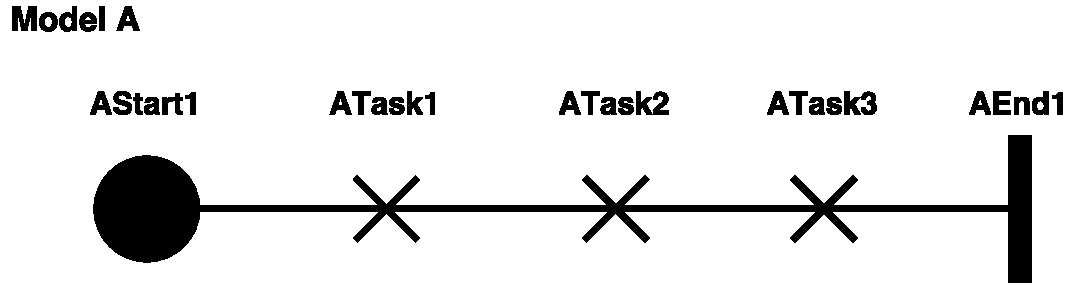
\includegraphics[scale=0.5]{fig_3_4.pdf}
	\caption{Example base scenario to be extended}
	\label{fig:3.4}
\end{figure}

\begin{figure}[h]
	\centering
	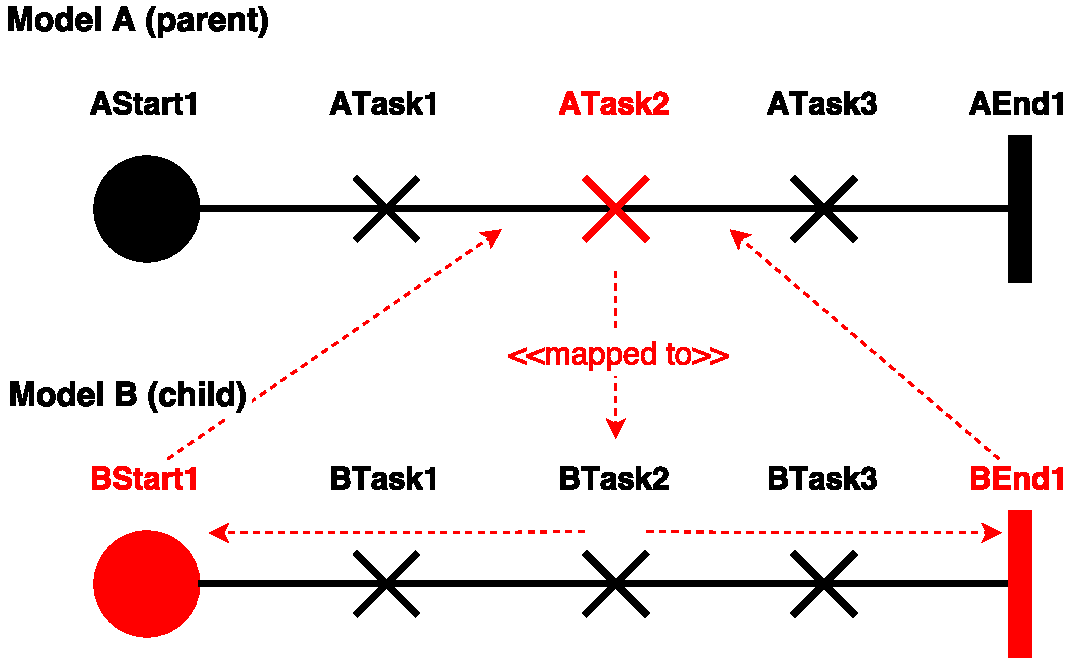
\includegraphics[scale=0.5]{fig_3_5.pdf}
	\caption{Schematic representation of extension with basic mapping}
	\label{fig:3.5}
\end{figure}

Furthermore, we allow multiple consecutive mappings between two UCM models (Figure~\ref{fig:3.6}). The path of a UCM may consist of mapped responsibilities interspersed with other path nodes. While traversing forward, lines~\ref{alg:1.16}-\ref{alg:1.17} handle the next mapped responsibility. If it exists, forward traversal stops for this specific composition and appropriate nodes are connected between \emph{UCM}\textsubscript{source} and \emph{UCM}\textsubscript{target}. For subsequent mappings, lines~\ref{alg:1.1}-\ref{alg:1.2} handle the linkage from previous mappings, and backward traversal stops at the point of mapped responsibilities and appropriate nodes are connected between \emph{UCM}\textsubscript{source} and \emph{UCM}\textsubscript{target}. This pattern continues until the weaver reaches an end point, whereby the predecessor of \emph{UCM}\textsubscript{target}'s end point connects to the successor of the mapped responsibility (\emph{from}) \emph{UCM}\textsubscript{source} and this end point is deleted (lines~\ref{alg:1.12}-\ref{alg:1.13}). Same goes for backward traversal until the weaver reaches a start point (lines~\ref{alg:1.5}-\ref{alg:1.6}). Lastly, the responsibility that was mapped (\emph{to}) in \emph{UCM}\textsubscript{target} remains in the model, while the responsibility that was mapped (\emph{from}) in \emph{UCM}\textsubscript{source} is deleted in the final woven UCM model.

\begin{figure}
	\centering
	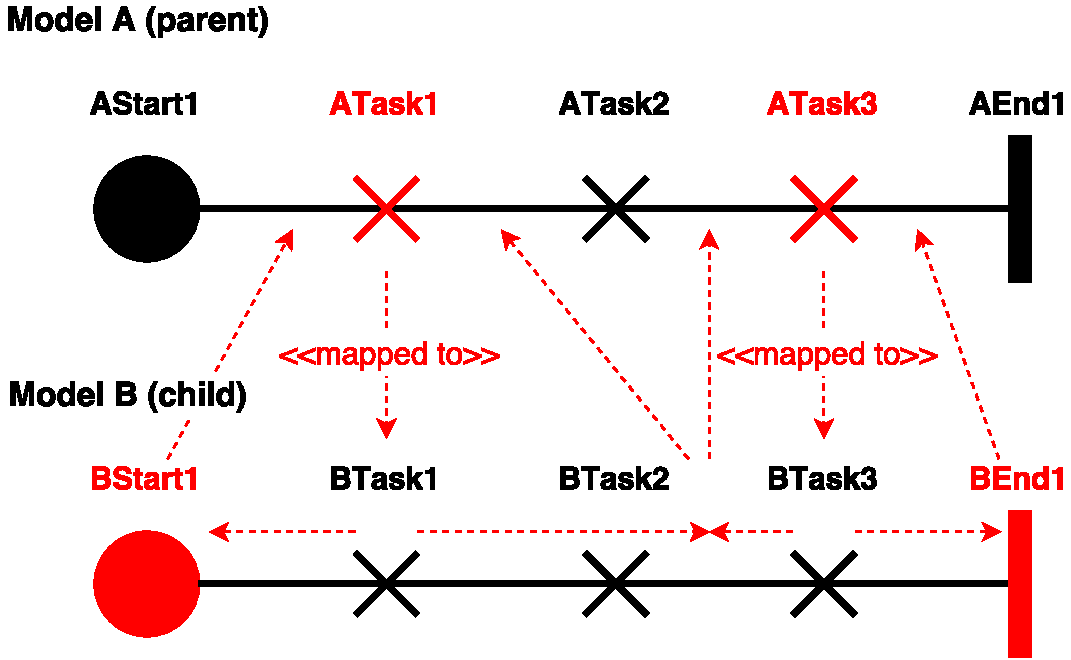
\includegraphics[scale=0.5]{fig_3_6.pdf}
	\caption{Schematic representation of extension with consecutive mappings}
	\label{fig:3.6}
\end{figure}

\begin{figure}[h]
	\centering
	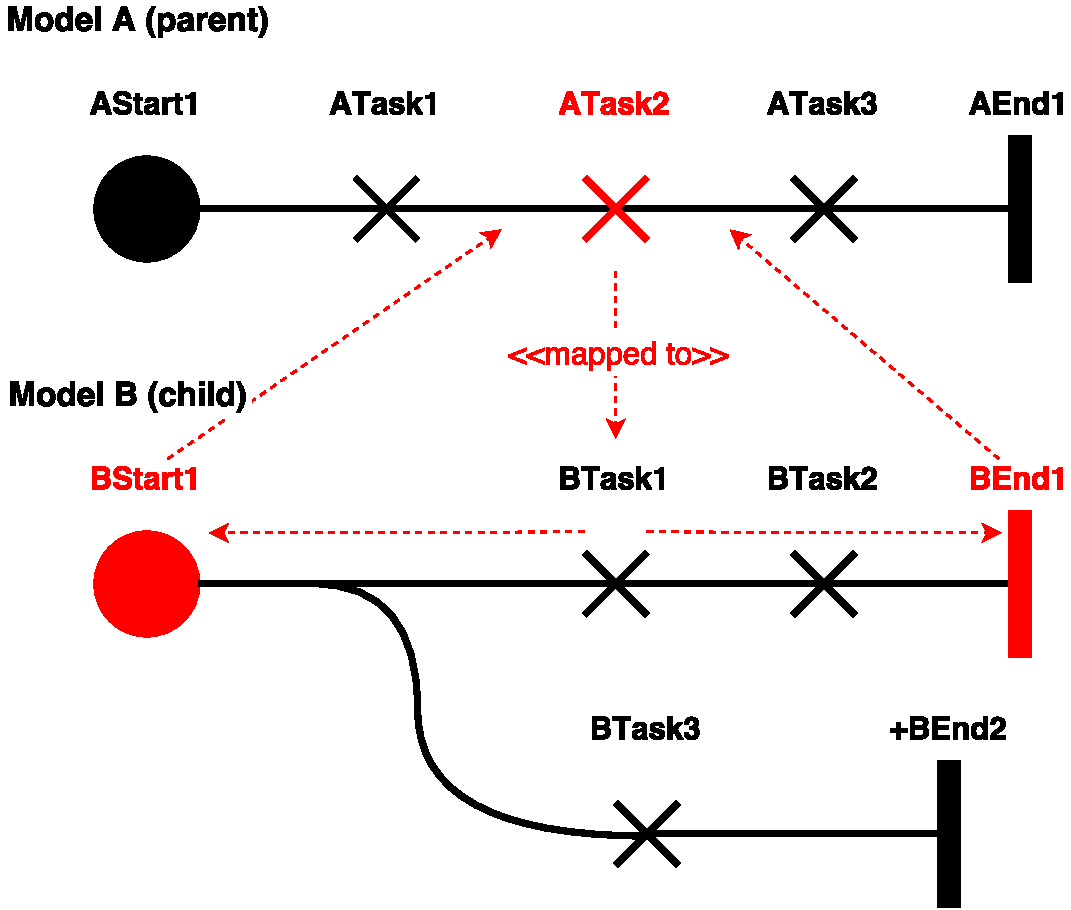
\includegraphics[scale=0.5]{fig_3_7.pdf}
	\caption{Schematic representation of extension with multiple branches}
	\label{fig:3.7}
\end{figure}

UCMs may have multiple start points joining into a path, or a path may branch to multiple end points (Figure~\ref{fig:3.7}). In this case, we allow a start or end point to set its visibility level. By default, a connecting point is given the visibility of {\cls Concern} that signifies the start or end point is only visible when viewing a UCM model for a specific feature of a concern, but disappears after the composition process. The other option is {\cls Public} for global visibility and is used to retain the start or end point even after the composition process---the weaver would just ignore {\cls Public} connecting points and proceed to other branches. This feature is useful in defining multiple entry points, or alternative exit strategies, for a scenario.

\begin{figure}[h]
	\centering
	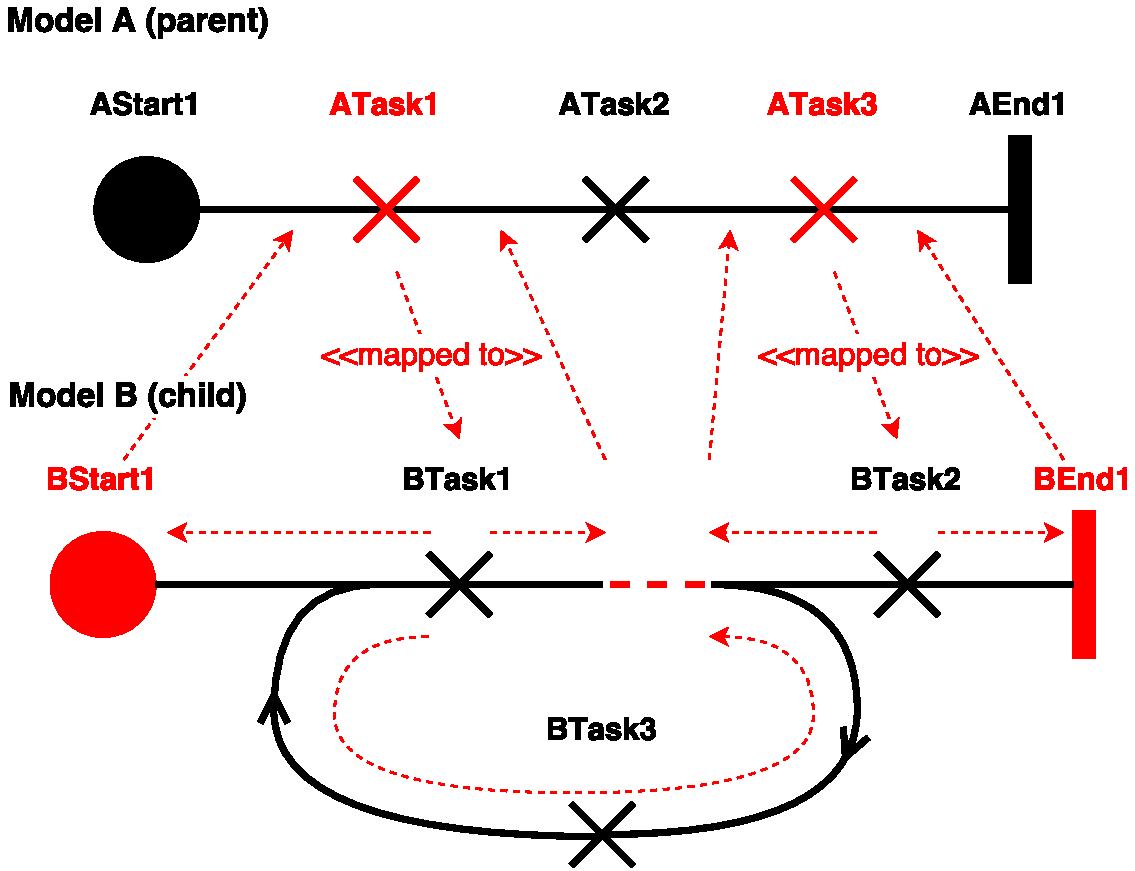
\includegraphics[scale=0.5]{fig_3_8.pdf}
	\caption{Schematic representation of extension with loop using anything node}
	\label{fig:3.8}
\end{figure}

Complex scenario model composition is also possible with the help of {\cls Anything}. An anything node can represent a subset of nodes in a path and is commonly used in \emph{UCM}\textsubscript{target} to capture the actual nodes that are specified in \emph{UCM}\textsubscript{source}. If an anything node is encountered during traversal, lines~\ref{alg:1.7}-\ref{alg:1.8} and~\ref{alg:1.14}-\ref{alg:1.15} signal the end of exploration and treat it as an end point. The difference is that the algorithm checks whether the anything node is still connected to other nodes before removal. This is necessary because an anything node has a predecessor node and a successor node, and typically surrounded by forks and joins to allow the insertion of loops in the base scenario (Figure~\ref{fig:3.8}). Both sides have to be traversed and dealt with before removing the anything node from the woven model.

\subsubsection{Connecting Point Mapping}

\begin{algorithm}
	\caption{Weaving Algorithm: Connecting Point Mapping}
	\label{alg:2}
	\begin{algorithmic}[1]
		\Function{WeaveConnectingPointMapping}{\emph{ucm}, \emph{composition}}
			\State \emph{node}\textsubscript{source} $\gets$ get first node of \emph{composition} mapping (\emph{from})
			\State \emph{node}\textsubscript{target} $\gets$ get second node of \emph{composition} mapping (\emph{to})
			\If{\emph{node}\textsubscript{source} is {\cls StartPoint}}
				\If{\emph{node}\textsubscript{source} is connected to a stub} \label{alg:2.1}
					\State call \Call{ExtendingStub\_Outgoing}{\emph{ucm}, \emph{node}\textsubscript{target}, \emph{node}\textsubscript{source}} \label{alg:2.2}
				\ElsIf{\emph{node}\textsubscript{target} is connected to a stub} \label{alg:2.3}
					\State call \Call{ReusingStub\_Incoming}{\emph{ucm}, \emph{node}\textsubscript{target}, \emph{node}\textsubscript{source}} \label{alg:2.4}
				\EndIf
			\ElsIf{\emph{node}\textsubscript{source} is {\cls EndPoint}}
				\If{\emph{node}\textsubscript{source} is connected to a stub} \label{alg:2.5}
					\State call \Call{ExtendingStub\_Incoming}{\emph{ucm}, \emph{node}\textsubscript{target}, \emph{node}\textsubscript{source}} \label{alg:2.6}
				\ElsIf{\emph{node}\textsubscript{target} is connected to a stub} \label{alg:2.7}
					\State call \Call{ReusingStub\_Outgoing}{\emph{ucm}, \emph{node}\textsubscript{target}, \emph{node}\textsubscript{source}} \label{alg:2.8}
				\EndIf
			\EndIf
		\EndFunction
		
		\Function{ExtendingStub\_Outgoing}{\emph{ucm}, \emph{node}\textsubscript{target}, \emph{node}\textsubscript{source}} \label{alg:2.9}
			\State \emph{node}\textsubscript{target\textsubscript{pred}} $\gets$ get predecessor node of \emph{node}\textsubscript{target}
			\State \emph{node}\textsubscript{source\textsubscript{pred}} $\gets$ get predecessor node of \emph{node}\textsubscript{source} via stub connection
			\State \emph{node}\textsubscript{source\textsubscript{succ}} $\gets$ get successor node of \emph{node}\textsubscript{source} via stub connection
			\State call \Call{MergePaths}{\emph{node}\textsubscript{target\textsubscript{pred}}, \emph{node}\textsubscript{source\textsubscript{pred}}, \emph{node}\textsubscript{source\textsubscript{succ}}, \emph{node}\textsubscript{source}, \emph{node}\textsubscript{source}}
			\State remove \emph{node}\textsubscript{target} from \emph{ucm}
		\EndFunction \label{alg:2.10}
		
		\Function{ReusingStub\_Incoming}{\emph{ucm}, \emph{node}\textsubscript{target}, \emph{node}\textsubscript{source}} \label{alg:2.11}
			\State \emph{node}\textsubscript{source\textsubscript{succ}} $\gets$ get successor node of \emph{node}\textsubscript{source}
			\State \emph{node}\textsubscript{target\textsubscript{succ}} $\gets$ get successor node of \emph{node}\textsubscript{target} via stub connection
			\State \emph{node}\textsubscript{target\textsubscript{pred}} $\gets$ get predecessor node of \emph{node}\textsubscript{target} via stub connection
			\State call \Call{SplitPaths}{\emph{node}\textsubscript{source\textsubscript{succ}}, \emph{node}\textsubscript{target\textsubscript{succ}}, \emph{node}\textsubscript{target\textsubscript{pred}}, \emph{node}\textsubscript{target}, \emph{node}\textsubscript{source}}
			\State remove \emph{node}\textsubscript{source} from \emph{ucm}
		\EndFunction \label{alg:2.12}
		
		\Function{ExtendingStub\_Incoming}{\emph{ucm} \emph{node}\textsubscript{target}, \emph{node}\textsubscript{source}} \label{alg:2.13}
			\State \emph{node}\textsubscript{target\textsubscript{succ}} $\gets$ get successor node of \emph{node}\textsubscript{target}
			\State \emph{node}\textsubscript{source\textsubscript{succ}} $\gets$ get successor node of \emph{node}\textsubscript{source} via stub connection
			\State \emph{node}\textsubscript{source\textsubscript{pred}} $\gets$ get predecessor node of \emph{node}\textsubscript{source} via stub connection
			\State call \Call{SplitPaths}{\emph{node}\textsubscript{target\textsubscript{succ}}, \emph{node}\textsubscript{source\textsubscript{succ}}, \emph{node}\textsubscript{source\textsubscript{pred}}, \emph{node}\textsubscript{source}, \emph{node}\textsubscript{source}}
			\State remove \emph{node}\textsubscript{target} from \emph{ucm}
		\EndFunction \label{alg:2.14}
		
		\algstore{alg2}
	\end{algorithmic}
\end{algorithm}

\begin{algorithm}                     
	\begin{algorithmic}[1]
		\algrestore{alg2}
		
		\Function{ReusingStub\_Outgoing}{\emph{ucm}, \emph{node}\textsubscript{target}, \emph{node}\textsubscript{source}} \label{alg:2.15}
			\State \emph{node}\textsubscript{source\textsubscript{pred}} $\gets$ get predecessor node of \emph{node}\textsubscript{source}
			\State \emph{node}\textsubscript{target\textsubscript{pred}} $\gets$ get predecessor node of \emph{node}\textsubscript{target} via stub connection
			\State \emph{node}\textsubscript{target\textsubscript{succ}} $\gets$ get successor node of \emph{node}\textsubscript{target} via stub connection
			\State call \Call{MergePaths}{\emph{node}\textsubscript{source\textsubscript{pred}}, \emph{node}\textsubscript{target\textsubscript{pred}}, \emph{node}\textsubscript{target\textsubscript{succ}}, \emph{node}\textsubscript{target}, \emph{node}\textsubscript{source}}
			\State remove \emph{node}\textsubscript{source} from \emph{ucm}
		\EndFunction \label{alg:2.16}
		
		\Function{SplitPaths}{\emph{node}\textsubscript{succ}, \emph{node}\textsubscript{succ}$'$, \emph{node}\textsubscript{pred}$'$, \emph{node}, \emph{node}$'$}
			\If{\emph{node}\textsubscript{succ}$'$ is {\cls Stub}} \label{alg:2.17}
				\State mark \emph{node}\textsubscript{succ}$'$ as removable stub
				\State set successor node of \emph{node}'s stub connection to \emph{node}\textsubscript{succ} \label{alg:2.18}
			\ElsIf{\emph{node}\textsubscript{succ}$'$ is {\cls AndFork} or {\cls OrFork}} \label{alg:2.19}
				\State create node connection between \emph{node}\textsubscript{succ}$'$ and \emph{node}\textsubscript{succ} \label{alg:2.20}
			\Else \label{alg:2.21}
				\State \emph{node}\textsubscript{stub} $\gets$ get successor node of \emph{node}$'$ via stub connection
				\State \emph{node}\textsubscript{fork} $\gets$ \textbf{if} \emph{node}\textsubscript{stub} is dynamic \textbf{then} create {\cls AndFork} \textbf{else} {\cls OrFork}
				\State place \emph{node}\textsubscript{fork} in between \emph{node}\textsubscript{pred}$'$ and \emph{node}\textsubscript{succ}$'$
				\State create node connection between \emph{node}\textsubscript{fork} and \emph{node}\textsubscript{succ}$'$
				\State create node connection between \emph{node}\textsubscript{fork} and \emph{node}\textsubscript{succ}
				\State set successor node of \emph{node}'s stub connection to \emph{node}\textsubscript{fork}
			\EndIf \label{alg:2.22}
		\EndFunction
		
		\Function{MergePaths}{\emph{node}\textsubscript{pred}, \emph{node}\textsubscript{pred}$'$, \emph{node}\textsubscript{succ}$'$, \emph{node}, \emph{node}$'$}
			\If{\emph{node}\textsubscript{pred}$'$ is {\cls Stub}} \label{alg:2.23}
				\State mark \emph{node}\textsubscript{pred}$'$ as removable stub
				\State set predecessor node of \emph{node}'s stub connection to \emph{node}\textsubscript{pred} \label{alg:2.24}
			\ElsIf{\emph{node}\textsubscript{pred}$'$ is {\cls AndJoin} or {\cls OrJoin}} \label{alg:2.25}
				\State create node connection between \emph{node}\textsubscript{pred} and \emph{node}\textsubscript{pred}$'$ \label{alg:2.26}
			\Else \label{alg:2.27}
				\State \emph{node}\textsubscript{stub} $\gets$ get predecessor node of \emph{node}$'$ via stub connection
				\State \emph{node}\textsubscript{join} $\gets$ \textbf{if} \emph{node}\textsubscript{stub} is synchronizing \textbf{then} create {\cls AndJoin} \textbf{else} {\cls OrJoin}
				\State place \emph{node}\textsubscript{join} in between \emph{node}\textsubscript{pred}$'$ and \emph{node}\textsubscript{succ}$'$
				\State create node connection between \emph{node}\textsubscript{pred}$'$ and \emph{node}\textsubscript{join}
				\State create node connection between \emph{node}\textsubscript{pred} and \emph{node}\textsubscript{join}
				\State set predecessor node of \emph{node}'s stub connection to \emph{node}\textsubscript{join}
			\EndIf \label{alg:2.28}
		\EndFunction
	\end{algorithmic}
\end{algorithm}

Mapping with connecting points allows for model extensions between parent and child UCMs and also model reuses from UCMs of other concerns. Algorithm~\ref{alg:2} illustrates the procedure of weaving for connecting point mappings. The function \emph{WeaveConnectingPointMapping} initiates the process by identifying the mapped connecting points (\emph{from} \emph{UCM}\textsubscript{source} \emph{to} \emph{UCM}\textsubscript{target}), and determining the type of composition to be performed based on whether the connecting points mapped from \emph{UCM}\textsubscript{source} are attached to a stub or not. If the mapped start and end points from \emph{UCM}\textsubscript{source} are attached to a stub (lines~\ref{alg:2.1}-\ref{alg:2.2} and~\ref{alg:2.5}-\ref{alg:2.6}), it means that the connecting points are hidden (Figure~\ref{fig:3.9}) and belong to a stub in \emph{UCM}\textsubscript{source} and are mapped to actual end and start points of \emph{UCM}\textsubscript{target}, respectively (cross mapping). This type of composition is model extension. For model reuse, the mapping is the inverse, i.e., the stub belongs to \emph{UCM}\textsubscript{target}, and the actual start and end points from \emph{UCM}\textsubscript{source} are mapped to it (lines~\ref{alg:2.3}-\ref{alg:2.4} and~\ref{alg:2.7}-\ref{alg:2.8}).

\begin{figure}[h]
	\centering
	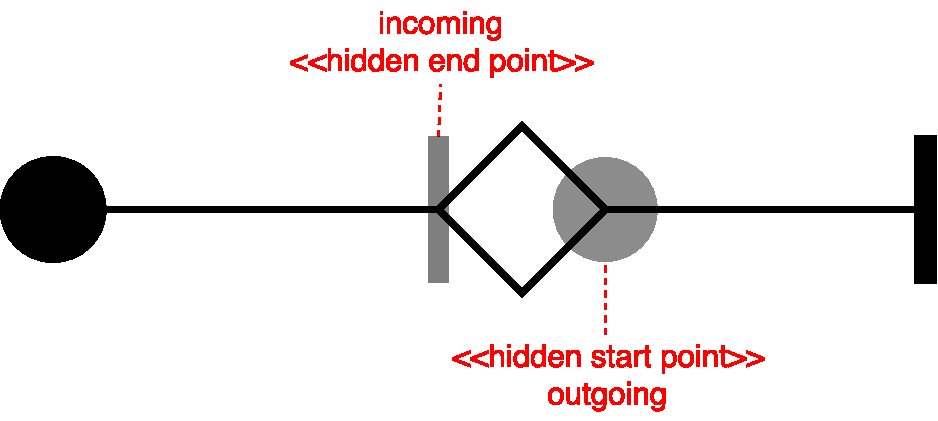
\includegraphics[scale=0.5]{fig_3_9.pdf}
	\caption{Example stub to indicate superimposed connecting points that are hidden}
	\label{fig:3.9}
\end{figure}

Model extension for stubs work differently compared with responsibilities. No traversal is required since there is no need to explore the whole graph, but the composition specification requires exactly two connecting point mappings for each stub to be complete---one for the start point and the second for the end point (Figure~\ref{fig:3.10}). The weaver first obtains the pair of mappings for the stub. The initial mapping usually maps the end point of a stub \footnote{The end point of a stub symbolizes incoming node connection to the stub.} to the start point of a UCM, and the weaver executes lines~\ref{alg:2.13}-\ref{alg:2.14}. The second mapping usually maps the start point of a stub \footnote{The start point of a stub symbolizes outgoing node connection from the stub.} to the end point of a UCM, and the weaver executes lines~\ref{alg:2.9}-\ref{alg:2.10}.

\begin{figure}[h]
	\centering
	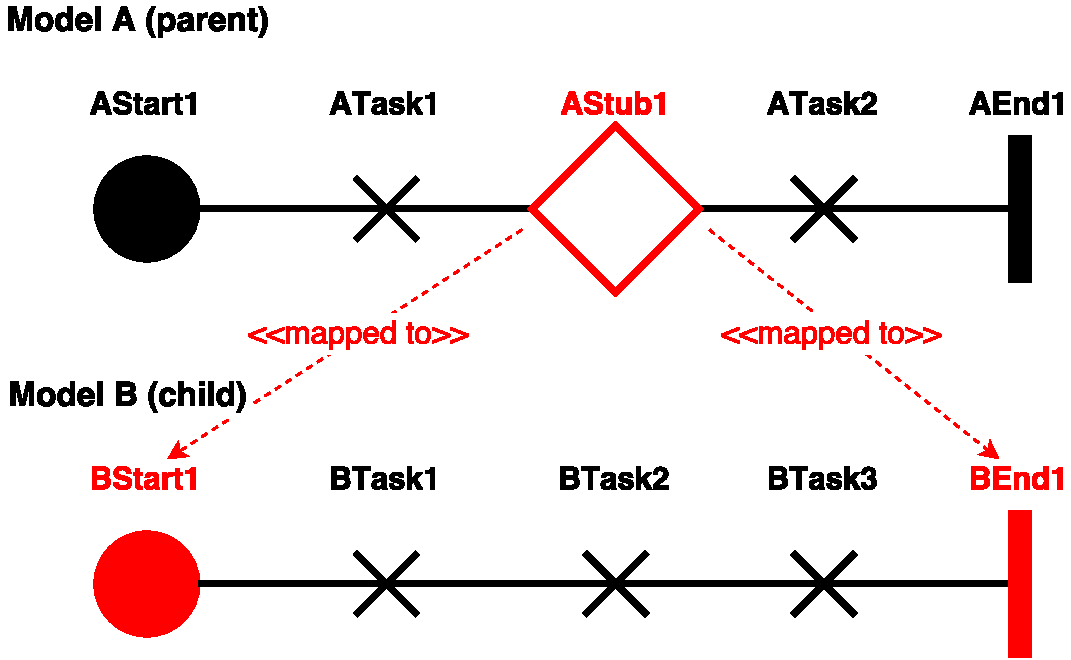
\includegraphics[scale=0.5]{fig_3_10.pdf}
	\caption{Schematic representation of extension through stub}
	\label{fig:3.10}
\end{figure}

As for model reuse, the order of mapping is reversed---start and end points of \emph{UCM}\textsubscript{source} are mapped to the connecting points of a stub that is automatically generated in \emph{UCM}\textsubscript{target} when reusing \emph{UCM}\textsubscript{source} (Figure~\ref{fig:3.11}). To be precise, the automatically generated stub is always a static stub so that it can only hold a single UCM that originates from the reused concern. The weaver then executes lines~\ref{alg:2.11}-\ref{alg:2.12} for mapping that maps from the start point of a UCM to the end point of a stub, and~\ref{alg:2.15}-\ref{alg:2.16} for mapping that maps from the end point of a UCM to the start point of a stub.

\begin{figure}[h]
	\centering
	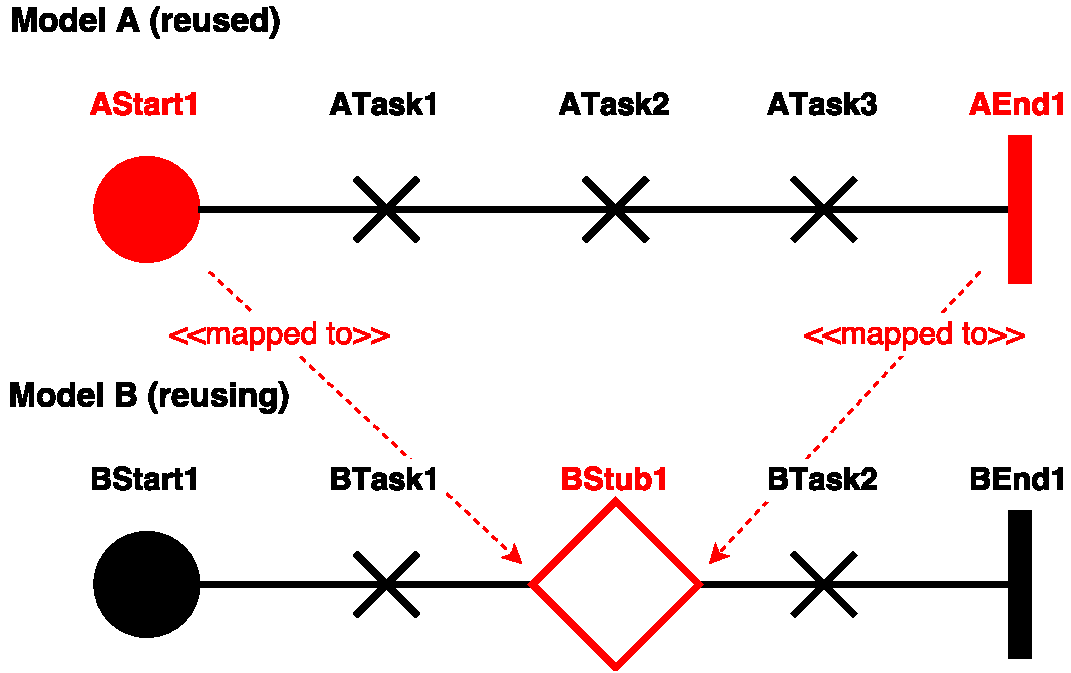
\includegraphics[scale=0.5]{fig_3_11.pdf}
	\caption{Schematic representation of reuse through stub}
	\label{fig:3.11}
\end{figure}

The execution procedure for both extension and reuse involves replacing a stub with plug-ins (sub-UCMs). Depending on the type of stub, it can bind either a single plug-in or multiple plug-ins. When facing a single plug-in bound to a stub, the weaver simply connects the nodes adjacent to the stub and nodes adjacent to the connecting points of a UCM, followed by the removal of the connecting points and the stub from the woven model (lines~\ref{alg:2.17}-\ref{alg:2.18} and~\ref{alg:2.23}-\ref{alg:2.24}). If there are two plug-ins bound to a stub, the weaver creates branches to link the two UCMs as parallel paths via fork and join nodes (lines~\ref{alg:2.21}-\ref{alg:2.22} and~\ref{alg:2.27}-\ref{alg:2.28}). The type of forks and joins being created is dependent on the type of stub. Synchronizing/blocking stubs produce branches that consist of {\cls AndFork} and {\cls AndJoin}, dynamic stubs produce branches that consist of {\cls AndFork} and {\cls OrJoin}, and static stubs produce branches that consist of {\cls OrFork} and {\cls OrJoin}. This process is also known as semantic flattening \cite{itu2012151}. Additional plug-ins bound to a stub are linked via the created forks and joins (lines~\ref{alg:2.19}-\ref{alg:2.20} and~\ref{alg:2.25}-\ref{alg:2.26}).
